\documentclass[article,A4,12pt]{llncs}
\usepackage[T1]{fontenc}
\usepackage{amsmath}
\usepackage{amssymb}
\usepackage{amsfonts}
\usepackage{mathrsfs, bm}

\usepackage{graphicx}
\usepackage{tabularx}
\usepackage{subfig}
\usepackage{epsf,times}
\usepackage{color}
\usepackage{wrapfig}
\usepackage{cases}
\usepackage{multicol}

\usepackage[T1]{fontenc}
%\newcommand{\tmname}[1]{\textsc{#1}}
%\newcommand{\tmop}[1]{\ensuremath{\operatorname{#1}}}
%\newcommand{\tmsamp}[1]{\textsf{#1}}
%\newcommand{\tmtextsc}[1]{{\scshape{#1}}}
%\newcommand{\tmtextsl}[1]{{\slshape{#1}}}
%\newcommand{\tmtexttt}[1]{{\ttfamily{#1}}}

\leftmargin=0.0cm
\oddsidemargin=0.5cm
\evensidemargin=0.5cm
\topmargin=0cm
\textwidth=16.0cm
%\textheight=21.5cm
\textheight=20.0cm
\pagestyle{plain}
\setlength{\columnsep}{20pt}

\def\m{\mathbf{m}}
\def\H{\mathbf{H}}
\def\E{\mathbf{E}}
\newcommand{\vepsi}{{\varepsilon}}
\def\hnorm#1#2{\vert\,#1\,\vert_{#2}}
\newcommand{\R}{{\mathbb R}}
\newcommand{\Sph}{{\mathbb S}}
\def\x{\mathbf{x}}
\def\hvec{\overline{\mathbf{h}}}
\def\evec{\overline{\mathbf{e}}}

\newcommand{ \etal}{\mbox{\emph{et al. }}}

\newcommand\vect[1]{\mbf{#1}}
\newcommand{\mbf}[1]{\mbox{\boldmath$#1$}} 
\newcommand{\RC}[1]{#1 $\times$ #1 $\times$ #1}
\def\um{$\mu$m}
\def\C{$^{\circ}\mathrm{C}$}

\newcommand{\Rmnum}[1]{\expandafter\@slowromancap\romannumeral #1@}

% DEFINITION OF CUSTOM FONT SIZE
\newcommand{\customfontA}{\fontsize{50}{55}\selectfont}
\newcommand{\customfontB}{\fontsize{14.4}{20}\selectfont}
\newcommand{\customfontC}{\fontsize{30}{35}\selectfont}

\DeclareMathAlphabet{\mathpzc}{OT1}{pzc}{m}{it}

\def\clovek#1{\noindent\bgroup\vbox{\noindent#1}\egroup\vskip1em}

% TO INPUT BACKGROUND IMAGE
\usepackage{eso-pic}
\newcommand\BackgroundPic{
\put(0,0){
\parbox[b][\paperheight]{\paperwidth}{
\vfill
\centering
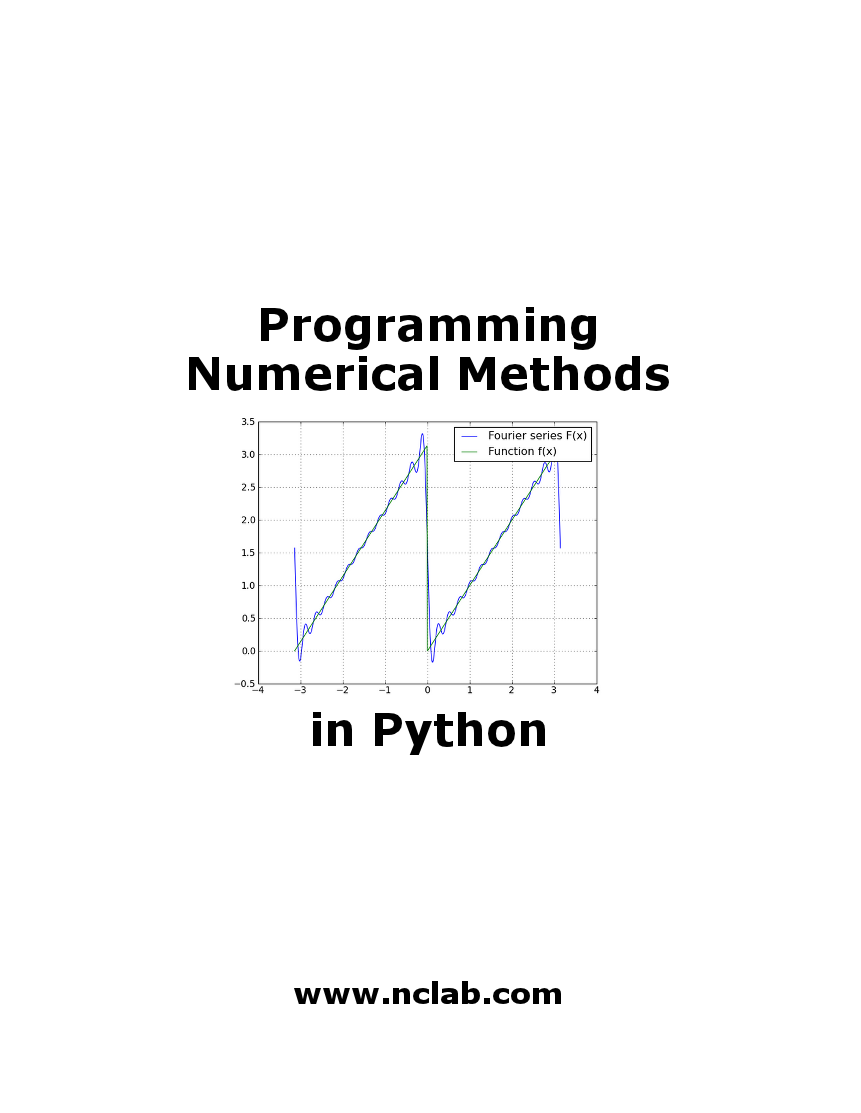
\includegraphics[width=\paperwidth,height=\paperheight]{img/numerical-frontpage.png}
%\includegraphics[width=\paperwidth,height=\paperheight]{img/background.jpg}
\vfill
}}}

\begin{document}

% INPUTTING BACKGROUND IMAGE
\AddToShipoutPicture{\BackgroundPic}
\vbox{}
\pagestyle{empty}
\newpage
\textwidth=15.5cm
\ClearShipoutPicture
\newpage

%%%%%%%%%%%%%%%%%%%%%%%%%%%%%%%%%%%%%%%%%%%%%%%%%%%%%%%%%%%%%%%%%%%%%%%%%

\section*{}
\small
\subsection*{About NCLab}
Networked Computing Laboratory (NCLab) is a popular Internet-based framework for 
programming, mathematics, computer modeling, 
and scientific computing. It serves students, instructors, researchers, and the general 
public. NCLab can be used free of charge for personal non-commercial purposes such as 
private hobby or self-education, as well as for individual non-funded academic research.
All other use is subject to {\bf purchasing a license} for a symbolic fee. The fees are as low as 
\$1 per user per month for educational use, and they are used to support the development 
and operational expenses. NCLab is a product of FEMhub Inc. The name "NCLab" is 
registered with the U.S. Patent and Trademark Office (USPTO) under Trademark No. 85420518.

\subsection*{Terms of Use and Pricing}
More details on purchasing a license and using NCLab are provided in the online documents 
{\bf Pricing} and {\bf Terms of Use} that are accessible from NCLab's home page 
{\tt http://nclab.com}.

\subsection*{Contact Information}
General inquiries: {\tt info@femhub.com}\\
Sales: {\tt sales@femhub.com}\\
NCLab support: {\tt support@nclab.com}\\
Agros \& Hermes support: {\tt support@femhub.com}\\
Web page: {\tt http://femhub.com}\\
{Physical address}\\
FEMhub Inc.\\
5490 Twin Creeks Dr.\\
Reno, NV 89523

\subsection*{About This Publication}
This publication can be copied and distributed without any restrictions
as long as reference to NCLab and FEMhub Inc. is preserved.


\normalsize

\newpage
%{\ }
\setcounter{tocdepth}{2}
\tableofcontents
%\pagestyle{plain}

\newpage

\pagestyle{plain}
\setcounter{page}{1}

%%%%%%%%%%%%%%%%%%%%%%%%%%%%%%%%%%%%%%%%%%%%%%%%%%%%%%%%%%%%%%%%%%%%%%%%%

\section{Introduction}

NCLab is a perfect place for instructors and students of Numerical Methods 
to experiment with numerical algorithms directly in classroom, use the methods
to solve real-world or training problems, as well as to do homework assignments. 
The list of programs that are readily available as Displayed Projects covers 
Numerical Methods I and Numerical Methods II as these courses are 
taught at most colleges and universities. \\

\noindent
This tutorial does not contain definitions, theorems and proofs. Instead, it 
gives examples of how the methods are used in practice, and it explains what 
their typical behavior is. The user can clone all programs into his/her account,
modify them and run as needed.
By going through this material and running the methods by yourself, you will 
gain a practical understanding of numerical methods that no textbook can give you. 

\section{Getting Started}

If NCLab is used as part of your Numerical Methods course, then you should 
have received a valid institution code. Use this code while creating 
and account and also for each login. If you are using NCLab for individual
non-commercial purposes, then you do not need an institution code (some 
limitations will apply, as described in Terms of Use). \\

\noindent
NCLab performs best 
with Chrome, Firefox, Safari and Opera browsers. Specifically, Internet Explorer
does not support some newer advanced visualization technologies used by NCLab 
and supported by other browsers. \\

\noindent
Before continuing, we recommend 
that you have a look at the introductory tutorial "Meet Your New Graphing 
Calculator" that explains how NCLab works and the best way to use it, as well as 
"Python Programming in Two Hours". You can also watch videos on the page 
http://femhub.com/nclab-tutorials/.\\

\noindent
After entering NCLab at {\tt http://nclab.com}, you will see a desktop with several icons on it,
as shown in Fig. \ref{fig:desktop}. 

\begin{figure}[!ht]
\begin{center}
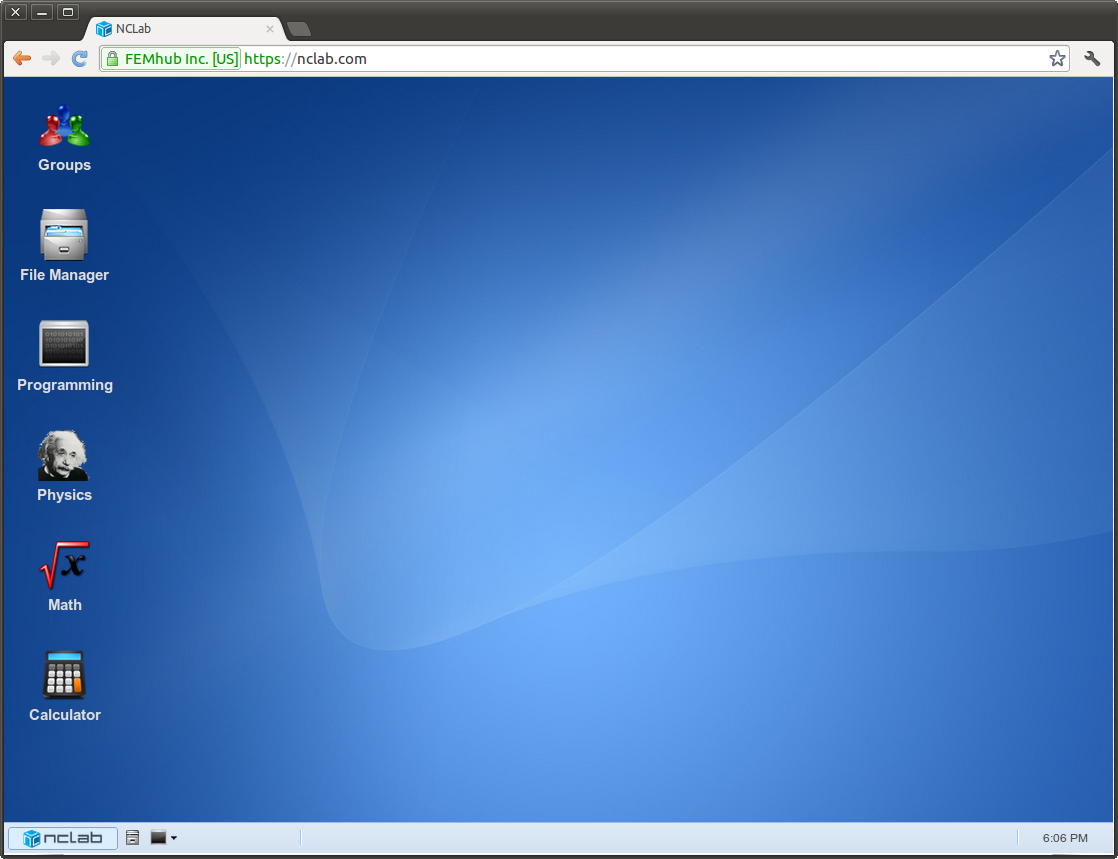
\includegraphics[width=\textwidth]{img/desktop.png}
\end{center}
%\vspace{-2mm}
\caption{NCLab desktop.}
\label{fig:desktop}
%\vspace{-1cm}
\end{figure}
\newpage
\noindent
The function of these icons is described, and a lot of other useful information for newcomers 
is provided in the introductory tutorial "Meet Your New Graphing Calculator". \\

\subsection{Cloning Displayed Projects}

All examples that we are going to work with are also available 
as Displayed Projects. You can clone them by launching the File
Manager, going to the {\em Project} menu, and clicking on {\em Clone}. This will launch 
a window with many displayed projects from various areas of programming,
math and computing. Look for projects whose names start with "Numerical Methods - 01",
"Numerical Methods - 02" and such.

After you locate a project that you would like to clone, click on it,
and then click on the button {\em Clone} at the bottom of the window. This will
create an exact copy of that project in your account, and you can open it 
by clicking on it in the File Manager. You can change the project in any way 
you like, the changes will not affect the original Displayed Project. 


\subsection{Launching a new Python project}

For those who prefer to do the programming by themselves: 
In the File Manager's {\em Project} menu 
choose {\em New} $\rightarrow$ {\em Python}. This will launch an 
empty Python project, as shown in Fig. \ref{fig:python}, and you can start 
programming right away. 

\begin{figure}[!ht]
\begin{center}
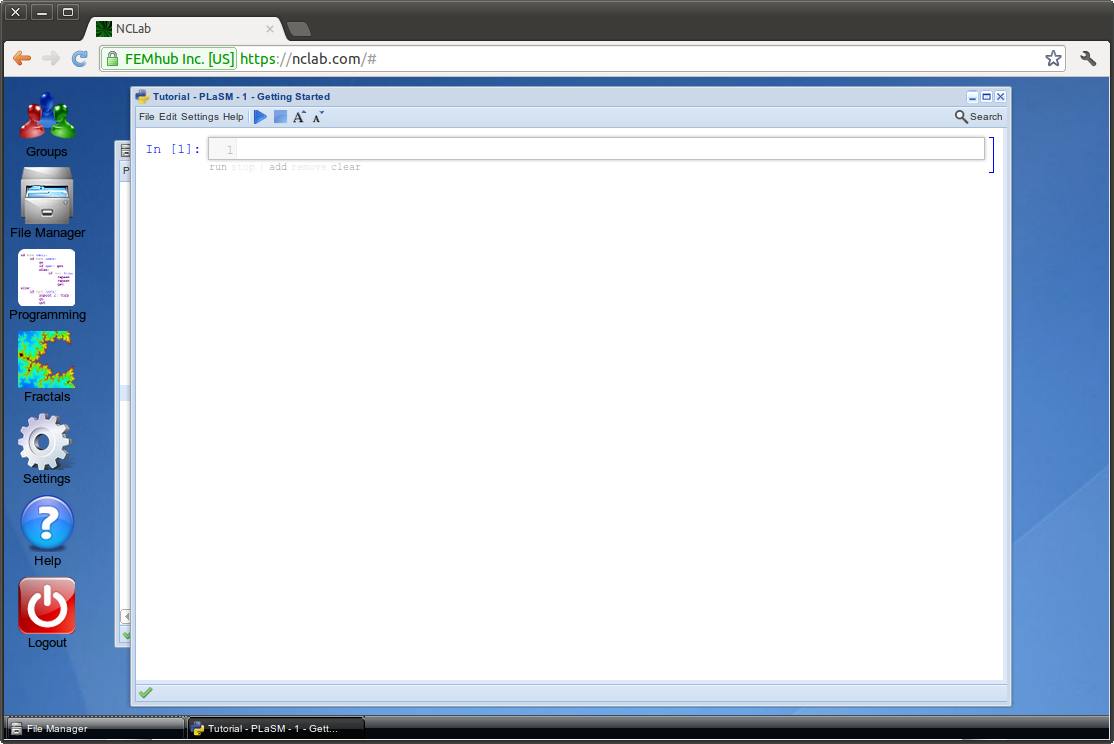
\includegraphics[width=\textwidth]{img/python.png}
\end{center}
%\vspace{-2mm}
\caption{Launching a new Python project.}
\label{fig:python}
\end{figure}
\noindent
All standard Python scientific  libraries are 
available, including Scipy, Numpy, Pylab, Matplotlib, and Sympy. 
The introductory tutorial "Meet Your New Graphing Calculator"
describes how to use NCLab to solve problems of high-school algebra,
calculus, matrix algebra and differential equations, how to 
plot graphs of functions of one and two variables, etc. 

GPU computing with PyCUDA is available for advanced users. There
is a separate tutorial on this topic, and many examples are provided
as Displayed Projects.


\newpage


\section{Warming Up}



\subsection{Finite computer arithmetic}

The following simple program demonstrates that the computer 
arithmetic is finite. If the computer stored numbers exactly 
as we know them from mathematics, then the condition in the while 
loop would be always satisfied, and the program would run forever:

\begin{verbatim}
# Finite computer arithmetics.
eps = 1.0
while 1.0 - eps < 1.0:
    print "eps =", eps
    eps /= 10.
print "Boom!"
\end{verbatim}
However, the output looks as follows:

\begin{verbatim}
eps = 1.0
eps = 0.1
eps = 0.01
eps = 0.001
eps = 0.0001
...
eps = 1e-15
eps = 1e-16
Boom!
\end{verbatim}
\noindent
So, the computer can't distinguish between $1$ and $1 - 10^{-17}$, these two numbers 
are the same in the computer arithmetic!

\subsection{Exercises}

\begin{enumerate}
\item The output displayed above corresponds to double-precision 
accuracy which is the default. Import from Numpy the function {\tt float32}
that converts numbers to single-precision accuracy, and inside the while loop,
convert {\tt 1.0 - eps} to single precision using {\tt float32(1.0 - eps)}.
How does the outcome of the program change?
\item It also follows from what we learned in this section that summation 
of infinite series using a computer is a tricky thing. It is well known,
for example, that the sum
$$
\sum_{n=1}^{\infty} \frac{1}{n}
$$
is infinite. Assuming that the computer would run an infinite loop, adding 
$1/n$ to the result in each step, at what $n$ would the value stop evolving 
in single and double precision arithmetic, and what would the result be?
\item Write a program that runs an infinite loop to calculate the sum
$$
\sum_{n=1}^{\infty} \frac{1}{n^6},
$$
but stop the program when you hit the finite computer accuracy and the result 
stops evolving (i.e., the result after adding the next increment does not 
change anymore). Compare the result 
obtained using the computer with the exact result. Do this in both double 
and single precision accuracy.
\end{enumerate}

\subsection{Absolute and relative error}

This example uses numerical differentiation to illustrate
absolute and relative error. We will differentiate the 
function 
$$
f(x) = 7e^{x/2}
$$
at the point $a = 2$. In this case the exact value is 
$$
f'(a) = \frac{7}{2}e^{a/2} \approx 9.51398639961.
$$
A numerical approximation $f'_{num}(a)$ of $f'(a)$ can be calculated using the differece
$$
f'_{num}(a) \approx \frac{f(a+h) - f(a)}{h}
$$
where $h$ is a small positive number. Let us choose, for example,
$h = 0.1$. Then $f'_{num}(a) = 9.75585027229$.\\

\noindent
The {\em true (absolute) error} is defined as the difference between the exact value and the approximation
(and take absolute value of that):
$$
err_{abs} = |f'(a) - f'_{num}(a)|.
$$
In our case $err_{abs} = 0.241863872682$. The {\em relative error} is defined by dividing 
the absolute error with the absolute value of the exact value -- of course this is only 
possible if the exact value is not zero:

$$
err_{rel} = \frac{|f'(a) - f'_{num}(a)|}{|f'(a)|}.
$$
In our case, $err_{rel} = 0.0254219275205$ which is $2.54219275205 \%$.

\subsection{Exercises}

\begin{enumerate}
\item Write a program that approximates the unit circle using an inscribed polygon 
      with $n$ equally-long sides, $n \ge 3$. The area of this polygon approximates the exact
      value of the area of the circle. Calculate the absolute and 
      relative error for an arbitrary $n$. Try to determine the power $\alpha$
      such that the error (any of the two) goes to zero as $1/n^{\alpha}$. The value 
      of $\alpha$ tells a lot about how good the method is. If $\alpha$ is low such 
      as $1$, the method is a {\em low-order method} (not too good). If $\alpha$ is
      higher than one, then the method is better and we call it a {\em higher-order method}.
      The higher the order of the method, the better, since we need a smaller $n$ to
      get an accurate approximation.
\item For $0 < q < 1$, it is 
      $$
      \frac{1}{1-q} = \sum_{n=0}^{\infty} q^n. 
      $$
      Write a program that takes as input the value of $q$ and a finite natural number 
      $m$. Instead of the infinite sum, calculate its approximation 
      $$
      \sum_{n=0}^{m} q^n. 
      $$ 
      Return the absolute and relative error of the approximation!
\item Do the same as in Exercise 2, but now approximate the infinite sum
      $$
      e^x = \sum_{n=0}^{\infty} \frac{x^n}{n!}
      $$
      The input for your program will be a real number $x$ and a natural number $m$.
      The output will be the absolute and relative errors.
\end{enumerate}


\subsection{Taylor polynomial}

Consider a given function $f(x)$ and an expansion point $a$. By {\em linear Taylor polynomial} $T_1(x)$ 
we mean a first-degree (i.e., linear) polynomial whose value $T_1(a) = f(a)$ and whose first derivative 
$T'_1(a) = f'(a)$. In other words, the graph of $T(x)$ is a tangent line to the graph of the function 
$f(x)$ at the point $[a, f(a)]$.
Of course, $f'(a)$ has to exist for $T_1(x)$ to be defined. 

Similarly, 
if $f''(a)$ exists, we can have a {\em quadratic Taylor polynomial} $T_2(x)$ satisfying
$T_2(a) = f(a)$, $T'_2(a) = f'(a)$, and $T''_2(a) = f''(a)$. And so on. 

The function that constructs a Taylor polynomial of an arbitrary degree $n$
symbolically is fairly simple:

\begin{verbatim}
def taylor_poly_symb(f, x, a, n):
    val = 0
    for i in range(n+1):
        val += f.subs(x, a)/factorial(i) * (x-a)**i
        f = f.diff(x)
    return val
\end{verbatim}
The main function {\tt taylor()} in example 03 - Taylor Polynomial in fact only calls the 
above six lines' script and the rest of it is plotting and error calculation. It is called 
with the following parameters:

\begin{verbatim}
taylor(a, f, x, n, xmin, xmax, subdiv)
\end{verbatim}
where {\tt a} is the expansion point, {\tt f} the function, {\tt x} the symbolic variable,
{\tt xmin} and {\tt xmax} the plotting interval, and {\tt subdiv} an optional parameter 
for plotting subdivision. Sample Taylor polynomials to $f(x) = e^x$ at $a = 0$
are shown in Figs. \ref{fig:taylor-1} - \ref{fig:taylor-3}.

\begin{figure}[!ht]
\begin{center}
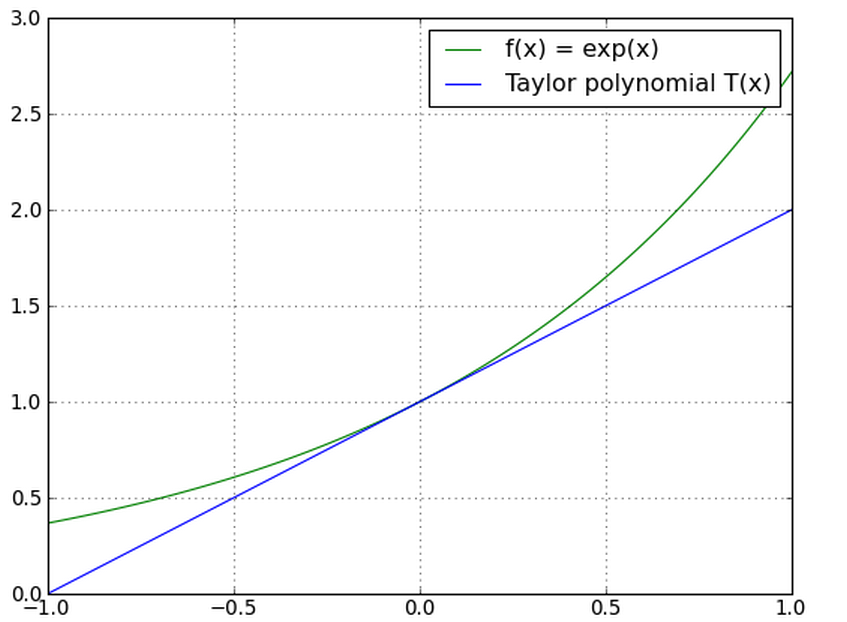
\includegraphics[width=0.6\textwidth]{img/taylor-1.png}
\end{center}
\vspace{-2mm}
\caption{Taylor polynomial $T_1(x) = 1+x$ of $f(x) = e^x$ at $a = 0$.}
\label{fig:taylor-1}
\end{figure}

\newpage

\begin{figure}[!ht]
\begin{center}
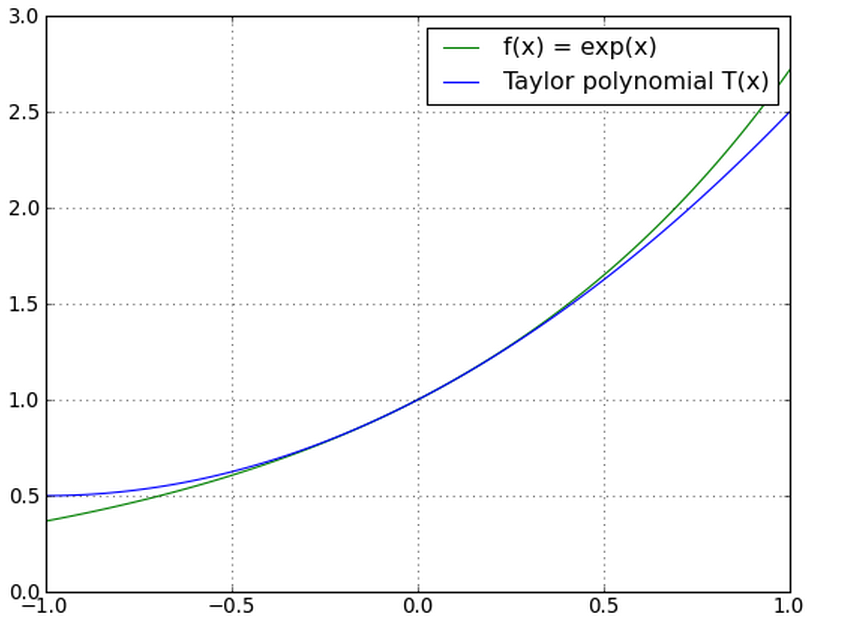
\includegraphics[width=0.6\textwidth]{img/taylor-2.png}
\end{center}
\vspace{-2mm}
\caption{Taylor polynomial $T_2(x) = 1+x+x^2/2$ of $f(x) = e^x$ at $a = 0$.}
\label{fig:taylor-2}
\vspace{6mm}
\end{figure}

\begin{figure}[!ht]
\begin{center}
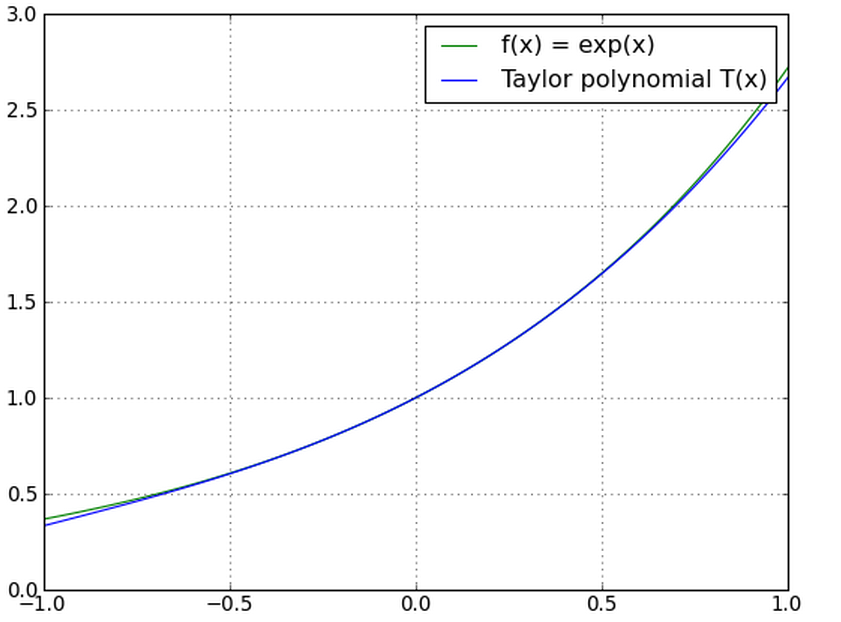
\includegraphics[width=0.6\textwidth]{img/taylor-3.png}
\end{center}
\vspace{-2mm}
\caption{Taylor polynomial $T_3(x) = 1+x+x^2/2+x^3/6$ of $f(x) = e^x$ at $a = 0$.}
\label{fig:taylor-3}
\end{figure}
\noindent
By numerical experimentation one can discover interesting facts that are not 
mentioned in numerical methods textbooks. One of them is that high-degree 
Taylor polynomials diverge very fast outside the are where they 
approximate the function $f$ nicely. This is illustrated in Fig. \ref{fig:taylor-4}.

\begin{figure}[!ht]
\begin{center}
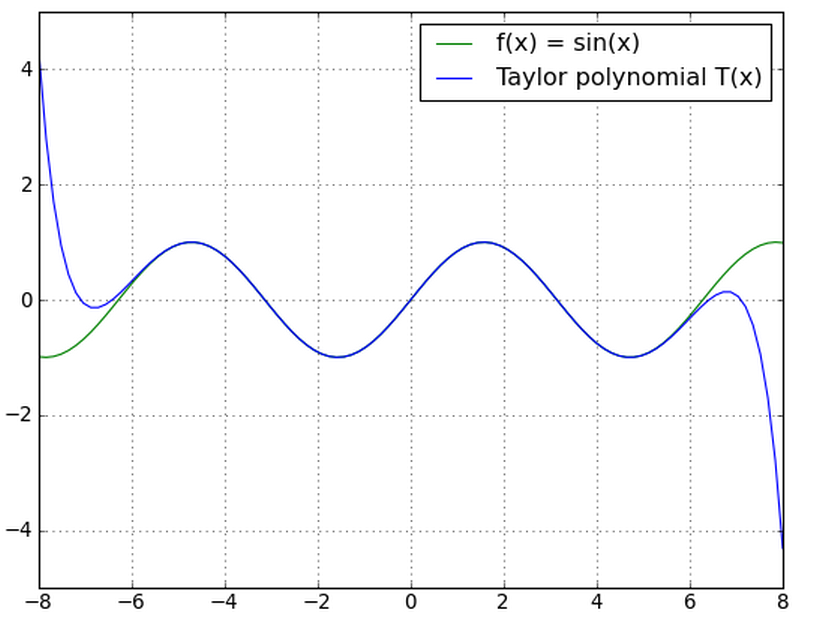
\includegraphics[width=0.6\textwidth]{img/taylor-4.png}
\end{center}
\vspace{-2mm}
\caption{Taylor polynomial $T_{15}(x)$ of $f(x) = \sin(x)$ at $a = 0$.}
\label{fig:taylor-4}
\end{figure}
\noindent
The effect shown in Fig.  \ref{fig:taylor-4} grows stronger as the degree 
$n$ of the polynomial increases. 

One important practical application of the Taylor polynomial is evaluation of 
frequently used functions such as $e^x$, $\sin(x)$, $\cos(x)$, $\log(x)$ 
in pocket calculators and computers. 
Other than that, Taylor polynomials are rarely used to solve practical problems.
But they are probably the most 
important technique of theoretical numerical analysis -- they are used to construct
the Newton's method (best method to solve nonlinear equations), to construct 
Runge-Kutta methods (most widely used methods to solve ordinary differential 
equations), as well as to analyze convergence of finite difference methods 
for partial differential equations and many other numerical methods. 

\subsection{Exercises}

\begin{enumerate}
\item Imagine that you are designing a calculator that is supposed to work in 
single precision arithmetic. Write a function {\tt exponential(x)} that will
use just the four basic operations {\tt +}, {\tt -}, {\tt *} and {\tt /} that 
are available in the calculator's processor, to approximate $e^x$ exactly to 8
decimal digits.
\item When solving engineering problems, very often (in fact always) we are 
looking to simplify our life. Sometimes this can be done by using a linear model instead of 
a nonlinear one. Sometimes by replacing a complicated function 
with a simpler one. For example, you task could be to solve equation $\cos(x) = x$
to the best of your ability. Looking at the graph and guessing are prohibited. 
You have to do it systematically. Hint: Replace $\cos(x)$ with its quadratic Taylor 
polynomial at $a = 0$. This will give you a surprizingly good approximation!
\item For the cases shown in Figs. \ref{fig:taylor-1} - \ref{fig:taylor-3}, the 
maximum values of $|f(x) - T_n(x)|$ in the interval 
$(-1, 1)$ were 0.718281828287, 0.218281828387 and 0.0516151617706, respectively.
Calculate the corresponding estimates using the Taylor Remainder Theorem, and compare
them with the true values! 
\end{enumerate}

\section{Solving Nonlinear Equations}




\subsection{Bisection method}



\subsection{Newton's method}

\subsection{Newton's method for systems}



\subsection{Fixed point method}


\subsection{Fixed point method with Anderson acceleration}

Anderson acceleration (sometimes called {\em Anderson mixing}) is a technique
to speed up the convergence of the fixed point method by considering 
a suitable linear combination of a few latest approximations, rather than 
just the latest approximation alone. 





\subsection{Solving polynomial equations with Numpy}





\section{Interpolation}





\subsection{Polynomial (Lagrange) interpolation}




\subsection{Interpolation with cubic splines}



\section{Matrix Methods}



\subsection{Dense and sparse matrix}


\subsection{Singular, nonsingular and inverse matrix}


\subsection{Condition number}


\subsection{LU factorization}


\subsection{Cholesky decomposition}


\subsection{Jacobi method}


\subsection{Gauss-Seidel method}


\subsection{SOR method}


\subsection{Steepest descent method}


\subsection{Modern iterative methods}


\subsection{COO to CSR conversion}


\subsection{CSR matrix-vector multiplications}


\subsection{Moore-Penrose inverse}




\section{Numerical Quadrature}


\subsection{Piecewise constant}


\subsection{Trapezoidal rule}


\subsection{Simpson's rule}


\subsection{Calculating weights}


\subsection{Arbitrary interval}


\subsection{Getting Gauss points and weights from Scipy}


\subsection{Gauss quadrature with $n$ points}


\subsection{Adaptive Gauss Quadrature}



\section{Approximation}


\subsection{Nonlinear regression}


\subsection{Linear regression}

\subsection{Least squares fit (continuous case)}


\subsection{Fourier series expansion}






\end{document}
